\section{Resultados}
Ao ser executado, o script LUA realizou as seguintes ações:
\begin{itemize}
\item Reconstrução da máquina síncrona no FEMM;
\item Definição do contorno;
\item Escolha dos materiais;
\item Definição do circuito elétrico;
\item Definição dos blocos (bobinas, material ferromagnético, ar);
\item Execução da função MESH (construção da malha de pontos);
\item Definição da linha de referência.
\item Construção do gráfico de densidade de fluxo magnético;
\item Construção do gráfico do potencial elétrico;
\item Construção do gráfico da da intensidade de campo;
\end{itemize}
%

\begin{figure}[H]
\centering
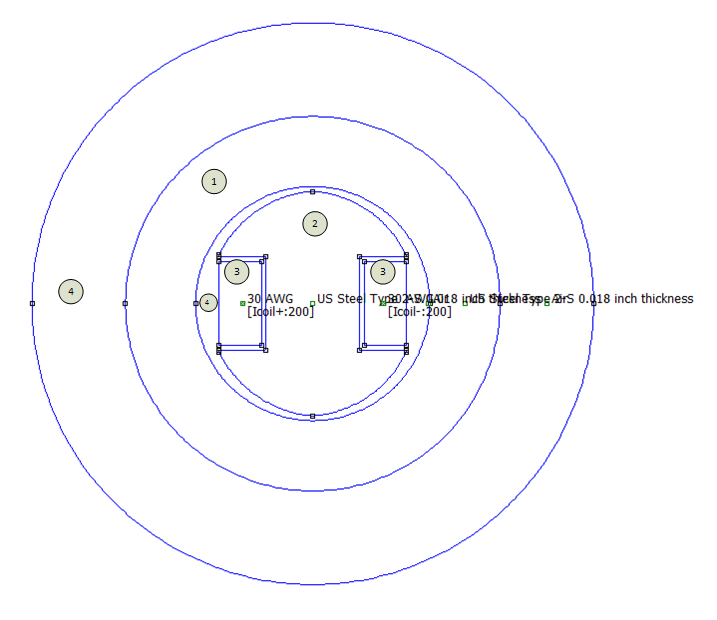
\includegraphics[scale=0.6]{img/assig4/femm_des.png}
\caption[Máquina rotativa]{Máquina rotativa: 1) Estator; 2) Rotor; 3) Enrolamento de campo; 4) Ar }
\label{}
\end{figure}

\begin{figure}[H]
\centering
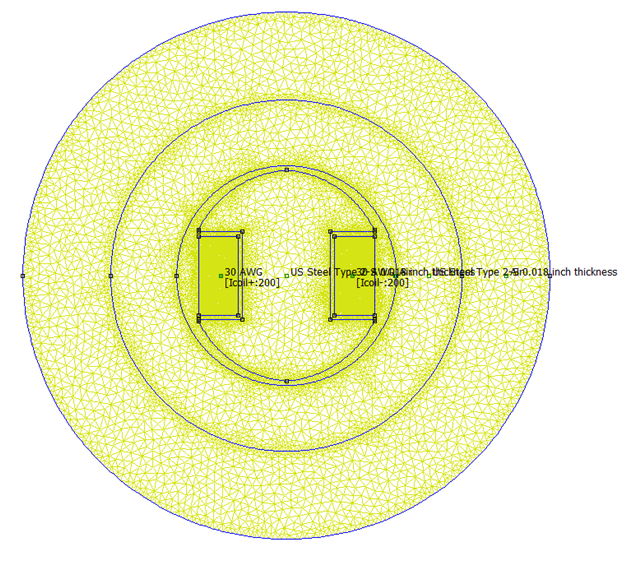
\includegraphics[scale=0.7]{img/assig4/triang.png}
\caption[Triangulação]{Triangulação}
\label{}
\end{figure}

\begin{figure}[H]
\centering
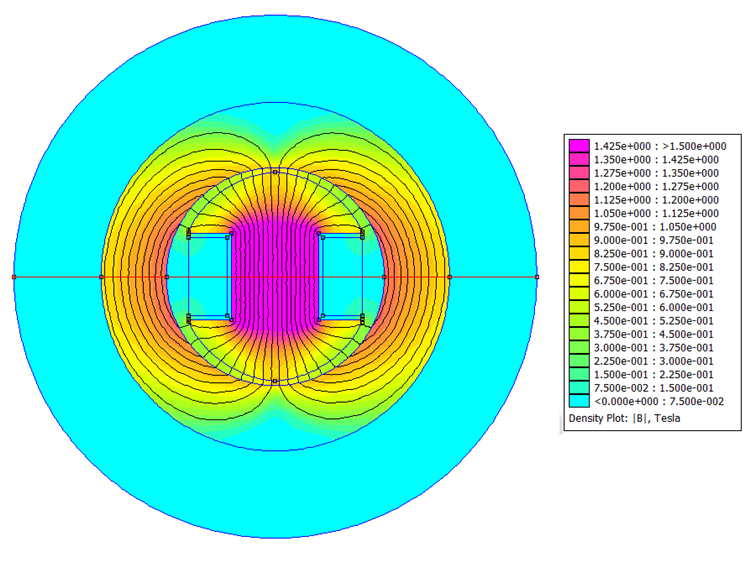
\includegraphics[scale=0.7]{img/assig4/femm_f.png}
\caption[Densidade de fluxo (Mapa de calor)]{Densidade de fluxo (Mapa de calor)}
\label{}
\end{figure}
%

A partir de uma linha horizontal, localizada em \textit{x = 0}, foram gerados os gráficos apresentados na figura \ref{grafs_4a}, \ref{grafs_4b} e \ref{grafs_4c}.
\begin{figure}[H]
\centering
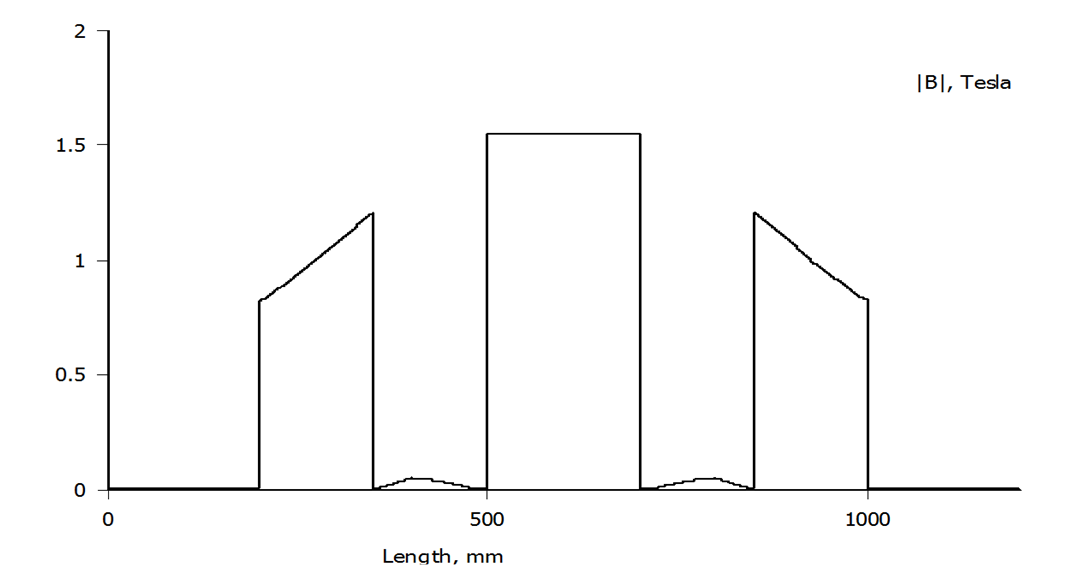
\includegraphics[scale=0.6]{img/assig4/femm_grafs_b.png}
\caption[Gráfico de densidade de fluxo magnético ]{Gráfico de densidade de fluxo magnético (|B|)}
\label{grafs_4a}
\end{figure}

\begin{figure}[H]
\centering
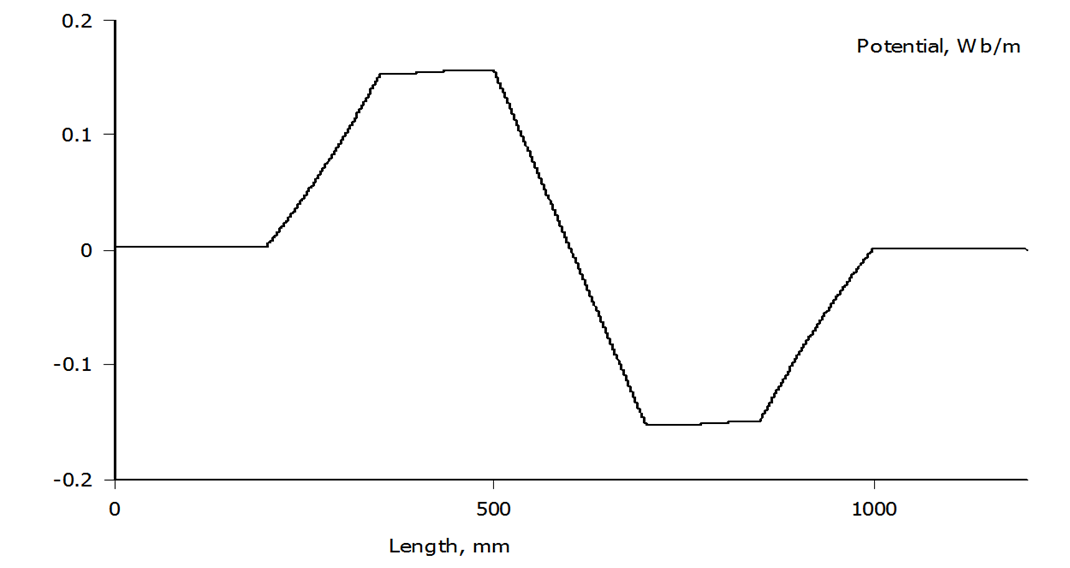
\includegraphics[scale=0.6]{img/assig4/femm_grafs_p.png}
\caption[Gráfico do potencial elétrico]{Gráfico do potencial elétrico}
\label{grafs_4b}
\end{figure}

\begin{figure}[H]
\centering
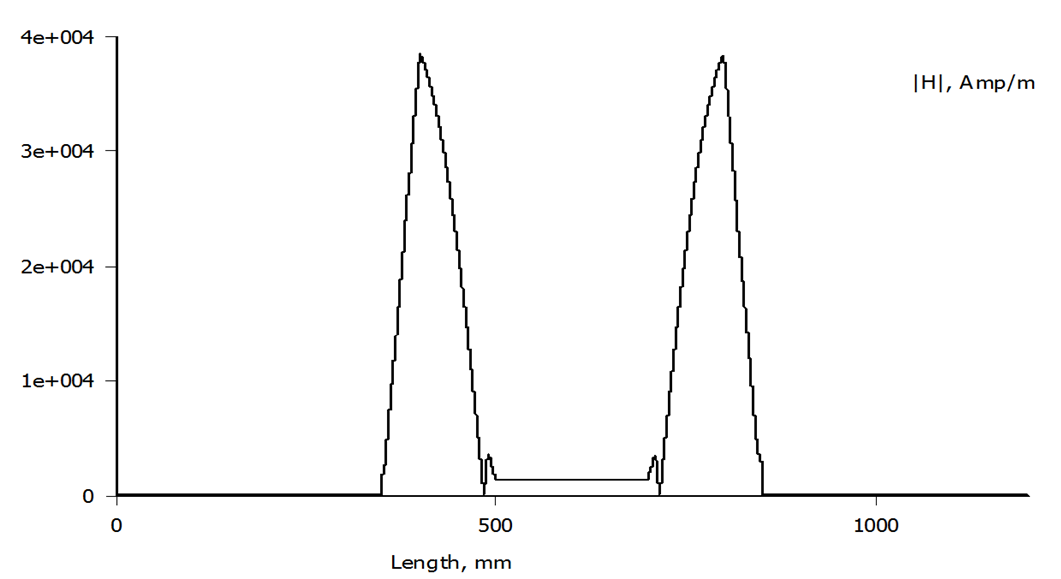
\includegraphics[scale=0.6]{img/assig4/femm_grafs_h.png}
\caption[Gráfico da intensidade de campo]{Gráfico da intensidade de campo (|H|)}
\label{grafs_4c}
\end{figure}
